\section{Theory}
\subsection*{Introduction}

In digital electronics, we deal with circuits in which there are only two states possible at any point, The \verb|HIGH| and \verb|LOW| voltage states represent the \verb|TRUE| and \verb|FALSE| states of Boolean logic.

When input signal is naturally discrete in nature, e.g., pulses from a particle detector, or \textit{bits} of data from a computer, the use of digital electronics is convenient. Furthermore, it is often desirable to convert analog data to digital form, and vice versa in order to perform computations on the data or to store large quantities of data as numbers.

Another advantage of digital techniques is the transmission of analog signals without
degradation by noise. An analog signal, picks up noise while being transmitted by cable or wireless that cannot be removed. If, instead, the signal is converted to a series of numbers representing its amplitude at successive instants of time, and these numbers are transmitted as digital signals, the analog signal reconstruction at
the receiving end will minimize error.
This technique is known as \text{pulse-code modulation}.

\subsection*{Logic Gates}

All digital electronic circuits and microprocessor based systems contain hardware elements called Digital Logic Gates that perform the logical operations of AND, OR and NOT on binary numbers.

Standard commercially available Digital Logic Gates are available in two basic forms, 

\begin{itemize}
    \item Transistor-Transistor Logic (TTL): 7400 series
    \item Complementary Metal-Oxide-Silicon (CMOS) 4000 series
\end{itemize}

These logic gates are embedded on Integrated Circuits (IC) or \textit{chips}. TTL IC's use NPN type Bipolar Junction Transistors while CMOS IC's use Field Effect Transistors or FET's for both their circuitry.\\

In digital circuitry, the voltage levels corresponding to \verb|HIGH| and \verb|LOW| are allowed to fall in some range, according to the particular logic family. For example, in a standard +5 volt supply, any TTL voltage input between 2V and
5V is considered to be \verb|HIGH| while any voltage input below 0.8V is
considered as \verb|LOW|. TTL outputs are recognized as \verb|LOW| between 0V and 0.4V and \verb|HIGH| between 2.7 V and 5 V. \\

\begin{figure}[H]
    \centering
    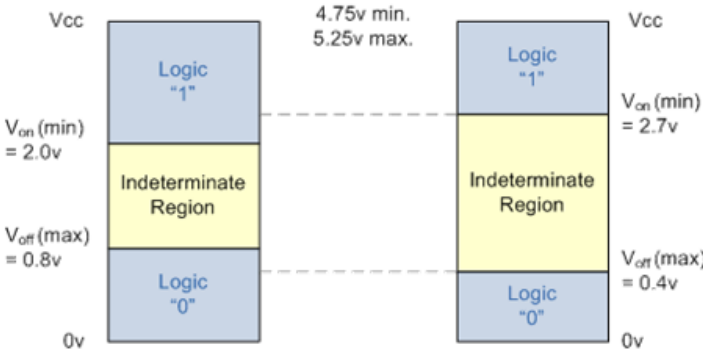
\includegraphics[width=0.75\columnwidth]{images/range.png}
    \caption{TTL Input \& Output Voltage Levels}
    \label{range}
\end{figure}

\noindent There are several types of simple logic gates.\\

\begin{itemize}
    \item \textbf{NOT Gate}: Also called an inverter, it takes one bit as input and produces output as its opposite. $Q=\overline{A}$
    
    \begin{figure}[!ht]
        \centering
        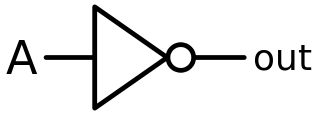
\includegraphics[width=0.30\columnwidth]{images/not.png}
        \qquad
        \begin{tabular}[b]{|c|c|}\hline
          A & Out \\ \hline
          1 & 0 \\
          0 & 1 \\ \hline
        \end{tabular}
        \caption{The circuit symbol and logic table for NOT gate}
    \end{figure}


    \item \textbf{OR Gate}: performs a logical OR operation on two inputs, A and B: $Q=A+B$.
    
    \begin{figure}[!ht]
        \centering
        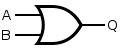
\includegraphics[width=0.30\columnwidth]{images/or.png}
        \qquad
        \begin{tabular}[b]{|c|c|c|}\hline
          A & B & Q \\ \hline
          0 & 0 & 0 \\ 
          0 & 1 & 1 \\
          1 & 0 & 1 \\
          1 & 1 & 1 \\ \hline
        \end{tabular}
        \caption{The circuit symbol and logic table for OR gate}
    \end{figure}


    \item \textbf{AND Gate}: performs a logical AND operation on two inputs, A and B: $Q=A\cdot B$.
    
    \begin{figure}[H]
        \centering
        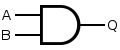
\includegraphics[width=0.30\columnwidth]{images/and.png}
        \qquad
        \begin{tabular}[b]{|c|c|c|}\hline
          A & B & Q \\ \hline
          0 & 0 & 0 \\ 
          0 & 1 & 0 \\
          1 & 0 & 0 \\
          1 & 1 & 1 \\ \hline
        \end{tabular}
        \caption{The circuit symbol and logic table for AND gate}
    \end{figure}
\end{itemize}

\noindent There are also two \textbf{Universal Gates}. These are combinations of an AND or an OR gate with a NOT gate.  

\begin{itemize}

    \item \textbf{NAND Gate}: Inverts AND operation: $Q=\overline{A \cdot B}$.
        
    \begin{figure}[H]
        \centering
        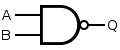
\includegraphics[width=0.30\columnwidth]{images/nand.png}
        \qquad
        \begin{tabular}[b]{|c|c|c|}\hline
        A & B & Q \\ \hline
        0 & 0 & 1 \\ 
        0 & 1 & 1 \\
        1 & 0 & 1 \\
        1 & 1 & 0 \\ \hline
        \end{tabular}
        \caption{The circuit symbol and logic table for NAND gate}
    \end{figure}

    \item \textbf{NOR Gate}: Inverts OR operation: $Q=\overline{A + B}$.
        
    \begin{figure}[H]
        \centering
        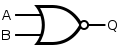
\includegraphics[width=0.30\columnwidth]{images/nor.png}
        \qquad
        \begin{tabular}[b]{|c|c|c|}\hline
        A & B & Q \\ \hline
        0 & 0 & 1 \\ 
        0 & 1 & 0 \\
        1 & 0 & 0 \\
        1 & 1 & 0 \\ \hline
        \end{tabular}
        \caption{The circuit symbol and logic table for NOR gate}
    \end{figure}
    
\end{itemize}

Thse gates can implement any Boolean function without need to use any other gate type. In practice, this is advantageous since NAND and NOR gates are economical and easier to fabricate and are the basic gates used in all IC digital logic families.

\begin{figure}[H]
    \centering
    \begin{subfigure}[b]{0.2\textwidth}
        \centering
        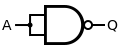
\includegraphics[width=\textwidth]{images/nand_not.png}
        \caption{NOT operation using NAND}
    \end{subfigure}
    \hfill
    \begin{subfigure}[b]{0.2\textwidth}
        \centering
        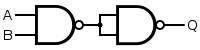
\includegraphics[width=\textwidth]{images/nand_and.png}
        \caption{AND operation using NAND}
    \end{subfigure}
    \hfill
    \begin{subfigure}[b]{0.2\textwidth}
        \centering
        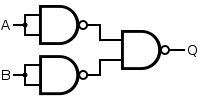
\includegraphics[width=\textwidth]{images/nand_or.png}
        \caption{OR operation using NAND}
    \end{subfigure}
    \hfill
       \caption{Other gates constructed using NAND}
       \label{nand}
    \end{figure}

\begin{figure}[H]
    \centering
    \begin{subfigure}[b]{0.2\textwidth}
        \centering
        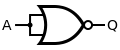
\includegraphics[width=\textwidth]{images/nor_not.png}
        \caption{NOT operation using NOR}
    \end{subfigure}
    \hfill
    \begin{subfigure}[b]{0.2\textwidth}
        \centering
        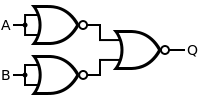
\includegraphics[width=\textwidth]{images/nor_and.png}
        \caption{AND operation using NOR}
    \end{subfigure}
    \hfill
    \begin{subfigure}[b]{0.2\textwidth}
        \centering
        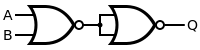
\includegraphics[width=\textwidth]{images/nor_or.png}
        \caption{OR operation using NOR}
    \end{subfigure}
    \hfill
       \caption{Other gates constructed using NOR}
       \label{nor}
\end{figure}

\noindent Additionally there are two more gates used.\\

\begin{itemize}

    \item \textbf{XOR Gate}: Exclusive OR, it outputs true if exclusively one of the inputs is true. Mathematically, $Q=A \cdot \overline{B} + B \cdot \overline{A} = A \oplus B$.
        
    \begin{figure}[H]
        \centering
        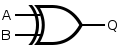
\includegraphics[width=0.30\columnwidth]{images/xor.png}
        \qquad
        \begin{tabular}[b]{|c|c|c|}\hline
        A & B & Q \\ \hline
        0 & 0 & 0 \\ 
        0 & 1 & 1 \\
        1 & 0 & 1 \\
        1 & 1 & 0 \\ \hline
        \end{tabular}
        \caption{The circuit symbol and logic table for XOR gate}
    \end{figure}

    \item \textbf{XNOR Gate}: Inverts XOR gate. Mathematically, $Q=A \cdot B + \overline{A} \cdot \overline{B} = A \odot B$.
        
    \begin{figure}[H]
        \centering
        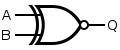
\includegraphics[width=0.30\columnwidth]{images/xnor.png}
        \qquad
        \begin{tabular}[b]{|c|c|c|}\hline
        A & B & Q \\ \hline
        0 & 0 & 1 \\ 
        0 & 1 & 0 \\
        1 & 0 & 0 \\
        1 & 1 & 1 \\ \hline
        \end{tabular}
        \caption{The circuit symbol and logic table for XNOR gate}
    \end{figure}
    
\end{itemize}

% ============================================================================

\subsection*{De Morgan's Laws}

De Morgan's laws, state that NAND gate is equivalent to an OR gate with negated inputs, and a NOR gate is equivalent to an AND gate with negated inputs. This is most commonly used to implement logic gates as combinations of only NAND gates, or as combinations of only NOR gates as shown in Fig. \ref{nand} \& \ref{nor}.

There are two basic theorems which can be proved using set theory. (Note: Here we use UNION and OR operators equivalently, as well as the INTERSECTION and AND operators).
\newpage

\noindent \textit{\textbf{Theorem 1: }}${\overline{A+B} = \overline{A} \cdot \overline {B}}$\\
\textit{\textbf{Proof: }} Using set theory,
\begin{gather*}
    \text{Let } x \in \overline{A \cup B}\\
    \implies x \notin (A \cup B) \\
    \implies x \notin A \text{ and } x \notin B\\
    \implies x \in \overline{A} \text{ and } x \in \overline{B}\\
    \implies x \in (\overline{A} \cap \overline{B})\,\,\,\forall\,x \in \overline{A \cup B}\\
    \text{or, }\overline{A} + \overline {B} = \overline{A \cdot B}
\end{gather*}

\noindent \textit{\textbf{Theorem 2: }}${\overline{A\cdot B} = \overline{A} + \overline {B}}$\\
\textit{\textbf{Proof: }} Using set theory,
\begin{gather*}
    \text{Let } y \in \overline{A \cap B}\\
    \implies y \notin (A \cap B) \\
    \implies y \notin A \text{ or } y \notin B \\
    \implies y \in \overline{A} \text{ or } y \in \overline{B}\\
    \implies y \in (\overline{A} \cup \overline{B})\,\,\,\forall\,y \in \overline{A \cap B}\\
    \text{or, }\overline{A} \cdot \overline {B} = \overline{A + B}
\end{gather*}

% ======================================================================================
\section{Experimental Setup}

\subsection*{Apparatus}

\begin{enumerate}
    \item Digital ICs
    \item Resistors
    \item DC Power Supply (5V)
    \item Breadboard
    \item Connecting Wires
    \item LEDs
\end{enumerate}

\subsection*{Circuit Diagrams}

\begin{figure}[H]
    \centering
    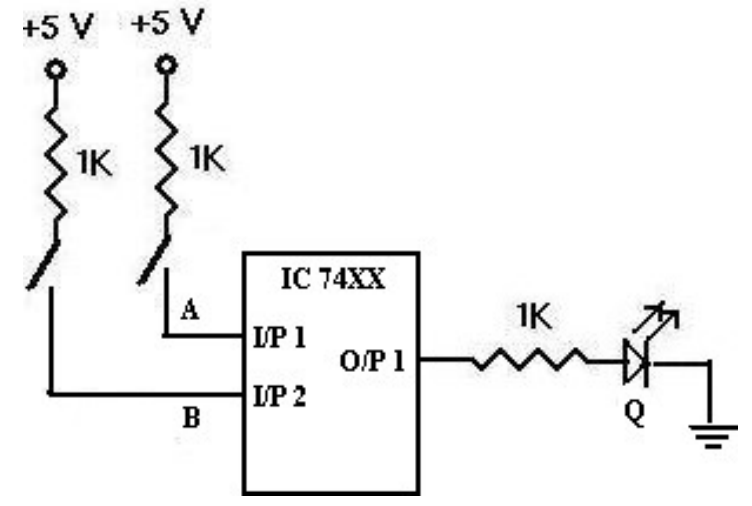
\includegraphics[width=0.60\columnwidth]{images/gen.png}
    \caption{General circuit diagram used for all the ICs}
    \label{gen}
\end{figure}

\begin{figure}[H]
    \centering
    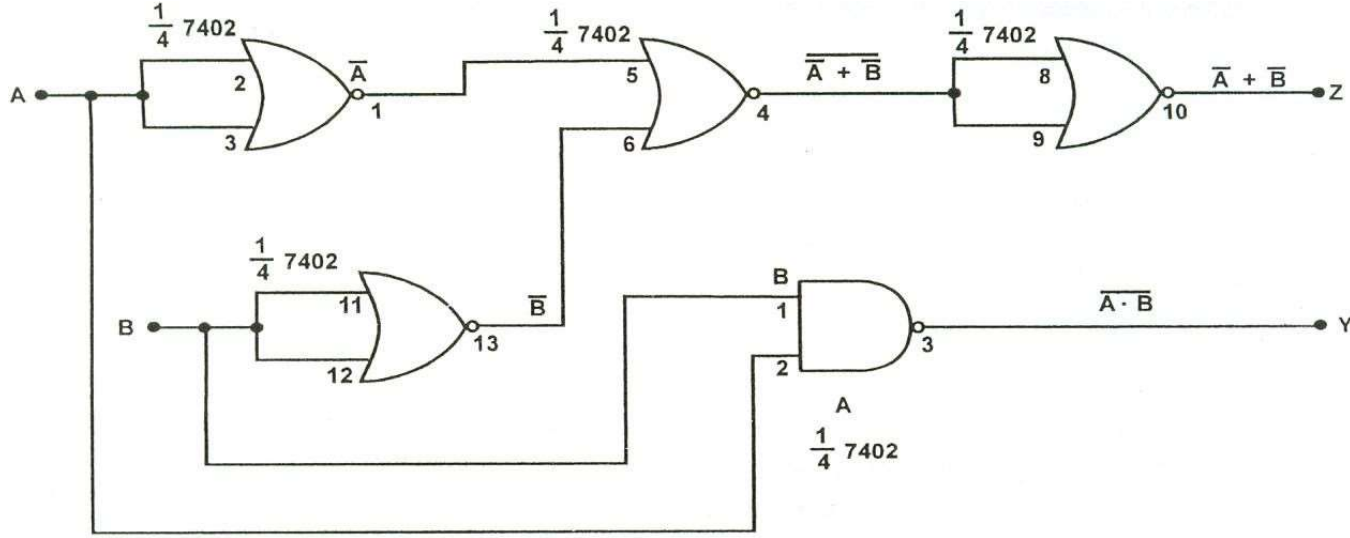
\includegraphics[width=1\columnwidth]{images/and_neg.png}
    \caption{Circuit diagram used for proving De Morgan's Law: ${\overline{A\cdot B} = \overline{A} + \overline {B}}$}
    \label{and_neg}
\end{figure}

\begin{figure}[H]
    \centering
    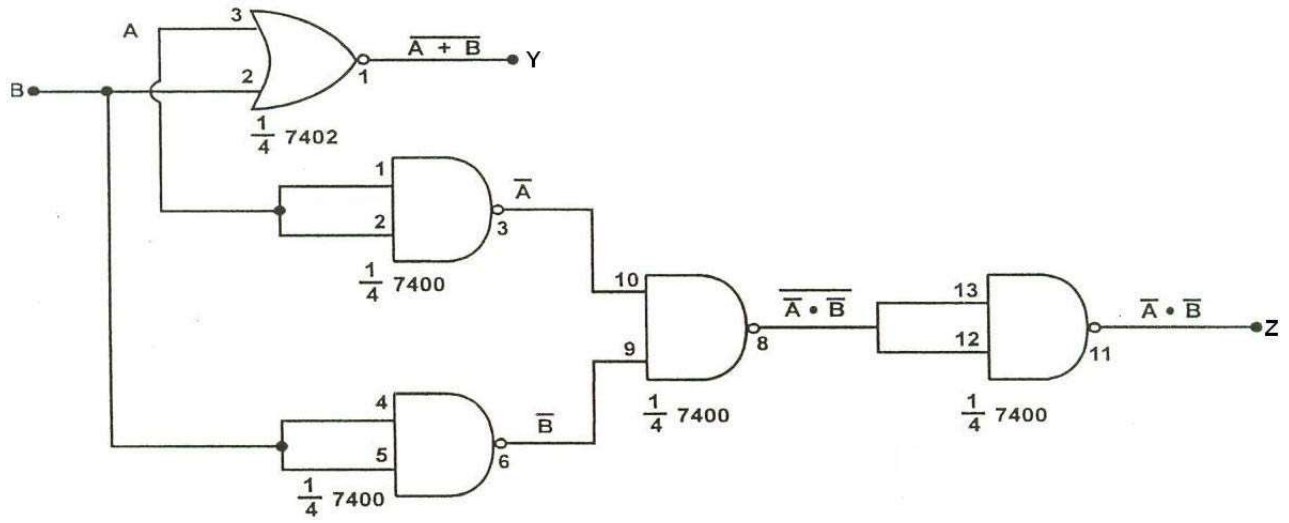
\includegraphics[width=1\columnwidth]{images/or_neg.png}
    \caption{Circuit diagram used for proving De Morgan's Law: ${\overline{A+B} = \overline{A} \cdot \overline {B}}$}
    \label{or_neg}
\end{figure}

\subsection*{IC Pinout Diagrams}

\begin{figure}[H]
    \centering
    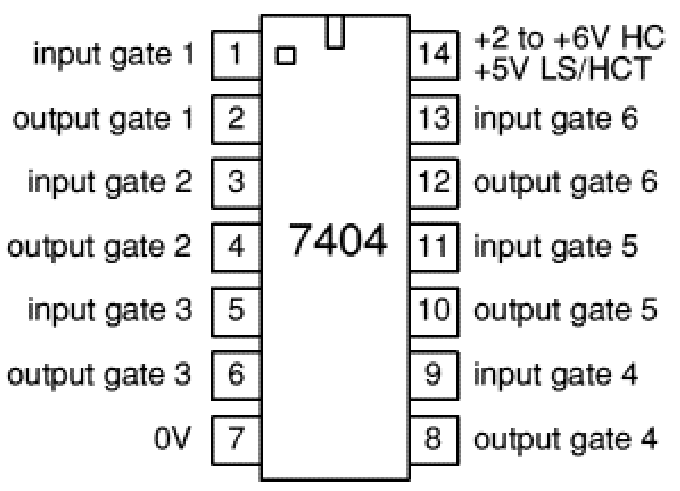
\includegraphics[width=0.6\columnwidth]{images/pinout_not.png}
    \caption{Pinout Diagram for NOT (IC 7404) gate. It contains 6 gates per IC.}
    \label{pinout1}
\end{figure}

\begin{figure}[H]
    \centering
    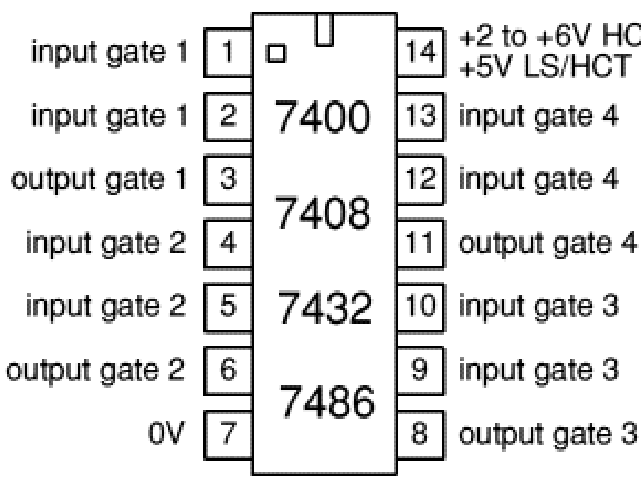
\includegraphics[width=0.6\columnwidth]{images/pinout_and.png}
    \caption{Pinout Diagram for AND (IC 7408), OR (IC 7432), XOR (IC 7486) and NAND (IC 7400) gates. Note how it contains only 4 gates per IC}
    \label{pinout2}
\end{figure}

\begin{figure}[H]
    \centering
    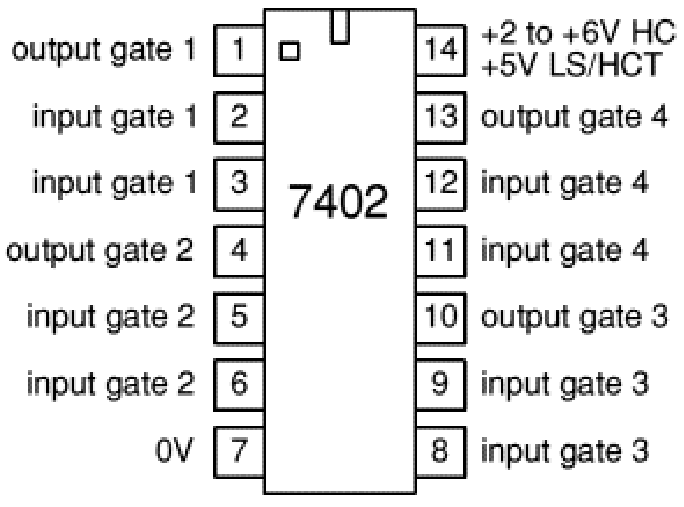
\includegraphics[width=0.6\columnwidth]{images/pinout_nor.png}
    \caption{Pinout Diagram for NOR (IC 7402) gate}
    \label{pinout3}
\end{figure}